\documentclass{ximera}

%% You can put user macros here
%% However, you cannot make new environments

\listfiles

\graphicspath{{./}{firstExample/}{secondExample/}}

\usepackage{tikz}
\usepackage{tkz-euclide}
\usepackage{tikz-3dplot}
\usepackage{tikz-cd}
\usetikzlibrary{shapes.geometric}
\usetikzlibrary{arrows}
\usetikzlibrary{decorations.pathmorphing,patterns}
\usetkzobj{all}
\pgfplotsset{compat=1.13} % prevents compile error.

\renewcommand{\vec}[1]{\mathbf{#1}}
\newcommand{\RR}{\mathbb{R}}
\newcommand{\dfn}{\textit}
\newcommand{\dotp}{\cdot}
\newcommand{\id}{\text{id}}
\newcommand\norm[1]{\left\lVert#1\right\rVert}
 
\newtheorem{general}{Generalization}
\newtheorem{initprob}{Exploration Problem}

\tikzstyle geometryDiagrams=[ultra thick,color=blue!50!black]

\usepackage{mathtools}

\title{Review of Power Series}%\label{Module 7-ADEF}


\begin{document}

\begin{abstract}

\end{abstract}

\maketitle

\section*{Review of Power Series}

Many applications give rise to differential equations with solutions
that can't be expressed in terms of elementary functions such as
polynomials, rational functions, exponential and logarithmic
functions, and trigonometric functions. The solutions of some of the
most important of these equations can be expressed in terms of power
series. We'll study such equations in this chapter. In this section
we review relevant properties of power series. We'll omit proofs,
which can be found in any standard calculus text.

\begin{definition}\label{thmtype:7.1.1}
An infinite series of the form
\begin{equation} \label{eq:7.1.1}
\sum_{n=0}^\infty a_n(x-x_0)^n,
\end{equation}
where $x_0$ and $a_0, a_1, \dots, a_n, \dots$ are constants, is
called a
\dfn{power series in} $x-x_0$. We say that the power series
\eqref{eq:7.1.1} \dfn{converges} for a given $x$ if the limit
$$
\lim_{N\rightarrow\infty}
\sum_{n=0}^Na_n(x-x_0)^n
$$
exists; otherwise, we say that the power series \dfn{diverges}  for
the given $x$.
\end{definition}

A power series in $x-x_0$ must converge if $x=x_0$, since the positive
powers of $x-x_0$ are all zero in this case. This may be the only
value of $x$ for which the power series converges. However, the
next theorem shows that if the power series converges for some
$x\neq
x_0$ then the set of all values of $x$ for which it converges forms an interval.

\begin{theorem}\label{thmtype:7.1.2}
For any power series
$$
\sum_{n=0}^\infty a_n(x-x_0)^n,
$$
exactly one of the these statements is true$:$
\begin{enumerate}
\item\label{item:7.1.2a} % (i)
The power series converges  only for $x=x_0.$
\item\label{item:7.1.2b} % (ii)
The power series converges for all values of $x.$
\item\label{item:7.1.2c} % (iii)
There's a positive number $R$ such that  the power series
converges if $|x-x_0|<R$ and diverges if  $|x-x_0|>R$.
\end{enumerate}
\end{theorem}


In case \ref{item:7.1.2c} we say that $R$ is the \dfn{radius of convergence} of
the power series. For convenience, we include the other two cases
in this definition by defining $R=0$ in case \ref{item:7.1.2a} and $R=\infty$ in
case \ref{item:7.1.2b}. We define the \dfn{open interval of convergence} of
$\sum_{n=0}^\infty a_n(x-x_0)^n$ to be
$$
 (x_0-R,x_0+R)\quad\mbox{if}\quad  0<R<\infty,\quad \mbox{or}\quad(-\infty,\infty) \quad\mbox{if}\quad R=\infty.
$$
If $R$ is finite, no general statement
can be made concerning convergence at the endpoints $x=x_0\pm R$ of
the open interval of convergence;   the series may converge at one or
both points, or diverge at both.


Recall from calculus that a series of constants
$\sum_{n=0}^\infty\alpha_n$ is said to \dfn{converge absolutely} if
the series of absolute values $\sum_{n=0}^\infty|\alpha_n|$ converges.
It can be shown that a power series $\sum_{n=0}^\infty a_n(x-x_0)^n$
with a positive radius of convergence $R$ converges absolutely in its
open interval of convergence; that is, the series
$$
\sum_{n=0}^\infty |a_n||x-x_0|^n
$$
of absolute values  converges if $|x-x_0|<R$. However, if $R<\infty$,
the series may fail to converge absolutely at an endpoint $x_0\pm R$,
even if it converges there.

The next theorem provides a useful method for determining the
radius of convergence of a power series. It's derived in calculus by
applying the ratio test to the corresponding series of absolute
values. 
%For related theorems see Exercises~\ref{exer:7.1.2} and
%\ref{exer:7.1.4}.

\begin{theorem}\label{thmtype:7.1.3}
Suppose there's an integer $N$ such that $a_n\ne0$ if
$n\geq N$ and
$$
\lim_{n\rightarrow\infty}\left|\frac{a_{n+1}}{a_n}\right|=L,
$$
where $0\leq L\leq \infty.$ Then the radius of convergence of
$\sum_{n=0}^\infty a_n(x-x_0)^n$ is $R=1/L,$ which should be interpreted
to mean that $R=0$ if $L=\infty,$ or $R=\infty$ if $L=0$.
\end{theorem}

\begin {example} \label{example:7.1.1}
 Find the radius of convergence of the series:
 \begin{enumerate}
\item\label{item:7.1.1a}
$\sum_{n=0}^\infty n!x^n$
\item\label{item:7.1.1b}
$\sum_{n=10}^\infty (-1)^n \frac{x^n}{n!}$
\item\label{item:7.1.1c}
$\sum_{n=0}^\infty 2^nn^2 (x-1)^n.$
\end{enumerate}

\begin{explanation}
\ref{item:7.1.1a}  Here $a_n=n!$, so
$$
\lim_{n\rightarrow\infty}\left|\frac{a_{n+1}}{a_n}\right|=\lim_{n\rightarrow\infty}
\frac{(n+1)!}{n!}=\lim_{n\rightarrow\infty}(n+1)=\infty.
$$
Hence, $R=0$.

\ref{item:7.1.1b}  Here $a_n=(1)^n/n!$ for $n\geq N=10$, so
$$
\lim_{n\rightarrow\infty}\left|\frac{a_{n+1}}{a_n}\right|=\lim_{n\rightarrow\infty}
\frac{n!}{(n+1)!}=\lim_{n\rightarrow\infty}\frac{1}{n+1}=0.
$$
Hence, $R=\infty$.

\ref{item:7.1.1c}  Here $a_n=2^nn^2$, so
$$
\lim_{n\rightarrow\infty}\left|\frac{a_{n+1}}{a_n}\right|=\lim_{n\rightarrow\infty}
\frac{2^{n+1}(n+1)^2}{2^nn^2}=2\lim_{n\rightarrow\infty}\left(1+\frac{1}{n}\right)^2=2.
$$
Hence, $R=1/2$.
\end{explanation}
\end{example}

\subsection*{Taylor Series}

If a function $f$ has derivatives of all orders at a point $x=x_0$,
then the
\href{http://www-history.mcs.st-and.ac.uk/Mathematicians/Taylor.html}{Taylor series of  $f$  about} $x_0$  is
defined by
$$
 \sum_{n=0}^\infty \frac{f^{(n)}(x_0)}{n!}(x-x_0)^n.
$$
In the special case where $x_0=0$, this series is also called the
\href{http://www-history.mcs.st-and.ac.uk/Mathematicians/Maclaurin.html}{Maclaurin series of} $f$.

 Taylor series for most of the common elementary
functions converge to the functions on their open intervals of
convergence. For example, you are probably  familiar with the
following Maclaurin series:
\begin{eqnarray}
e^x&=&\sum_{n=0}^\infty \frac{x^n}{n!},\quad
-\infty<x<\infty,\label{eq:7.1.2}\\
\sin x&=&\sum_{n=0}^\infty(-1)^n \frac{x^{2n+1}}{(2n+1)!},\quad
-\infty<x<\infty, \label{eq:7.1.3}\\ %dummy \eqref{eq:7.1.3}
\cos x&=&\sum_{n=0}^\infty(-1)^n \frac{x^{2n}}{(2n)!},\quad
-\infty<x<\infty, \label{eq:7.1.4}\\ %dummy \eqref{eq:7.1.4}
\frac{1}{1-x}&=&\sum_{n=0}^\infty x^n,\quad-1<x<1.\label{eq:7.1.5}
\end{eqnarray}

\subsection*{Differentiation of Power Series}

A power series with a positive radius of convergence defines a
function
$$
f(x)=\sum_{n=0}^\infty a_n(x-x_0)^n
$$
on its open interval of convergence. We say that the series \dfn{represents} $f$ on the open interval of convergence. A function $f$
represented by a power series may be a familiar elementary function
as in  \eqref{eq:7.1.2}--\eqref{eq:7.1.5};     however, it often happens
that
$f$ isn't  a familiar function,  so  the series actually \dfn{defines}  $f$.

The next  theorem shows  that a  function represented  by a power
series  has  derivatives  of  all  orders  on  the  open  interval  of
convergence  of   the  power   series,  and   provides  power  series
representations of the derivatives.

\begin{theorem}\label{thmtype:7.1.4}
A power series
$$
f(x)=\sum_{n=0}^\infty a_n(x-x_0)^n
$$
with positive radius of convergence $R$ has derivatives of all orders
in its open interval of convergence, and successive  derivatives
can be obtained by repeatedly differentiating term by term; that is,
\begin{eqnarray}
f'(x)&=&\sum_{n=1}^\infty
na_n(x-x_0)^{n-1}\label{eq:7.1.6},\\
f''(x)&=&\sum_{n=2}^\infty
n(n-1)a_n(x-x_0)^{n-2},\label{eq:7.1.7}\\
&\vdots&\nonumber\\
f^{(k)}(x)&=&\sum_{n=k}^\infty
n(n-1)\cdots(n-k+1)a_n(x-x_0)^{n-k}\label{eq:7.1.8}.
\end{eqnarray}
Moreover, all of these series have the same radius of convergence $R$.
\end{theorem}

\begin{example}\label{example:7.1.2}
Let $f(x)=\sin x$. From \eqref{eq:7.1.3},
$$
f(x)=\sum_{n=0}^\infty(-1)^n \frac{x^{2n+1}}{(2n+1)!}.
$$
From  \eqref{eq:7.1.6},
$$
f'(x)=\sum_{n=0}^\infty(-1)^n\frac{d}{dx}\left[\frac{x^{2n+1}}{(2n+1)!}\right]=
\sum_{n=0}^\infty(-1)^n \frac{x^{2n}}{(2n)!},
$$
which is the series  \eqref{eq:7.1.4} for $\cos x$.
\end{example}

\subsection*{Uniqueness of Power Series}

The next theorem shows that if $f$ is \dfn{defined} by a power
series in $x-x_0$ with a positive radius of convergence, then the power
series is the Taylor series of $f$ about $x_0$.

\begin{theorem}\label{thmtype:7.1.5}
If the power series
$$
f(x)=\sum_{n=0}^\infty a_n(x-x_0)^n
$$
has a positive radius of convergence, then
\begin{equation} \label{eq:7.1.9}
a_n=\frac{f^{(n)}(x_0)}{n!};
\end{equation}
that is, $\sum_{n=0}^\infty a_n(x-x_0)^n$ is the Taylor
series of $f$ about $x_0$.
\end{theorem}

This result can be obtained by setting $x=x_0$ in
\eqref{eq:7.1.8}, which yields
$$
f^{(k)}(x_0)=k(k-1)\cdots1\cdot a_k=k!a_k.
$$
This implies that
$$
a_k=\frac{f^{(k)}(x_0)}{k!}.
$$
Except for notation, this is the same as \eqref{eq:7.1.9}.

The next theorem lists two important properties of power series
that follow from Theorem~\ref{thmtype:7.1.5}.

\begin{theorem}\label{thmtype:7.1.6}
\begin{enumerate}
\item\label{item:7.1.6a} % (a)
If
$$
\sum_{n=0}^\infty a_n(x-x_0)^n=\sum_{n=0}^\infty b_n(x-x_0)^n
$$
for all $x$  in an open interval that contains $x_0,$ then
$a_n=b_n$ for $n=0, 1, 2, \dots$.
\item\label{item:7.1.6b} % (b)
If
$$
\sum_{n=0}^\infty a_n(x-x_0)^n=0
$$
 for all $x$ in
an open interval that contains $x_0,$ then $a_n=0$ for
$n=0, 1, 2, \dots$.
\end{enumerate}
\end{theorem}

To obtain \ref{item:7.1.6a} we observe that the two series represent the same function $f$ on the open  interval; hence, Theorem~\ref{thmtype:7.1.5}
implies that
$$
a_n=b_n=\frac{f^{(n)}(x_0)}{n!},\quad n=0,1,2, \dots.
$$
Part \ref{item:7.1.6b}  can be obtained from \ref{item:7.1.6a} by taking $b_n=0$ for
$n=0, 1, 2, \dots$.

\subsection*{Taylor Polynomials}

If $f$ has $N$ derivatives at a point $x_0$, we say that
$$
T_N(x)=\sum_{n=0}^N\frac{f^{(n)}(x_0)}{n!}(x-x_0)^n
$$
is the
\href{http://www-history.mcs.st-and.ac.uk/Mathematicians/Taylor.html}{$N$-th Taylor polynomial of $f$ about $x_0$}.
This definition and Theorem~\ref{thmtype:7.1.5} imply  that if
$$
f(x)=\sum_{n=0}^\infty a_n(x-x_0)^n,
$$
where the power series has a positive radius of convergence,
then the Taylor polynomials of $f$ about $x_0$ are given by
$$
T_N(x)=\sum_{n=0}^N a_n(x-x_0)^n.
$$
In numerical applications, we use the Taylor polynomials to
approximate $f$ on subintervals of the open interval of convergence of
the power series. For example,  \eqref{eq:7.1.2} implies that the Taylor
polynomial $T_N$ of $f(x)=e^x$ is
$$
T_N(x)=\sum_{n=0}^N\frac{x^n}{n!}.
$$
The solid curve in the figure below is the graph
of $y=e^x$ on the interval $[0,5]$. The  dotted curves
in the figure are the graphs of the Taylor polynomials
$T_1, \dots, T_6$ of $y=e^x$ about $x_0=0$. 

\begin{image}
 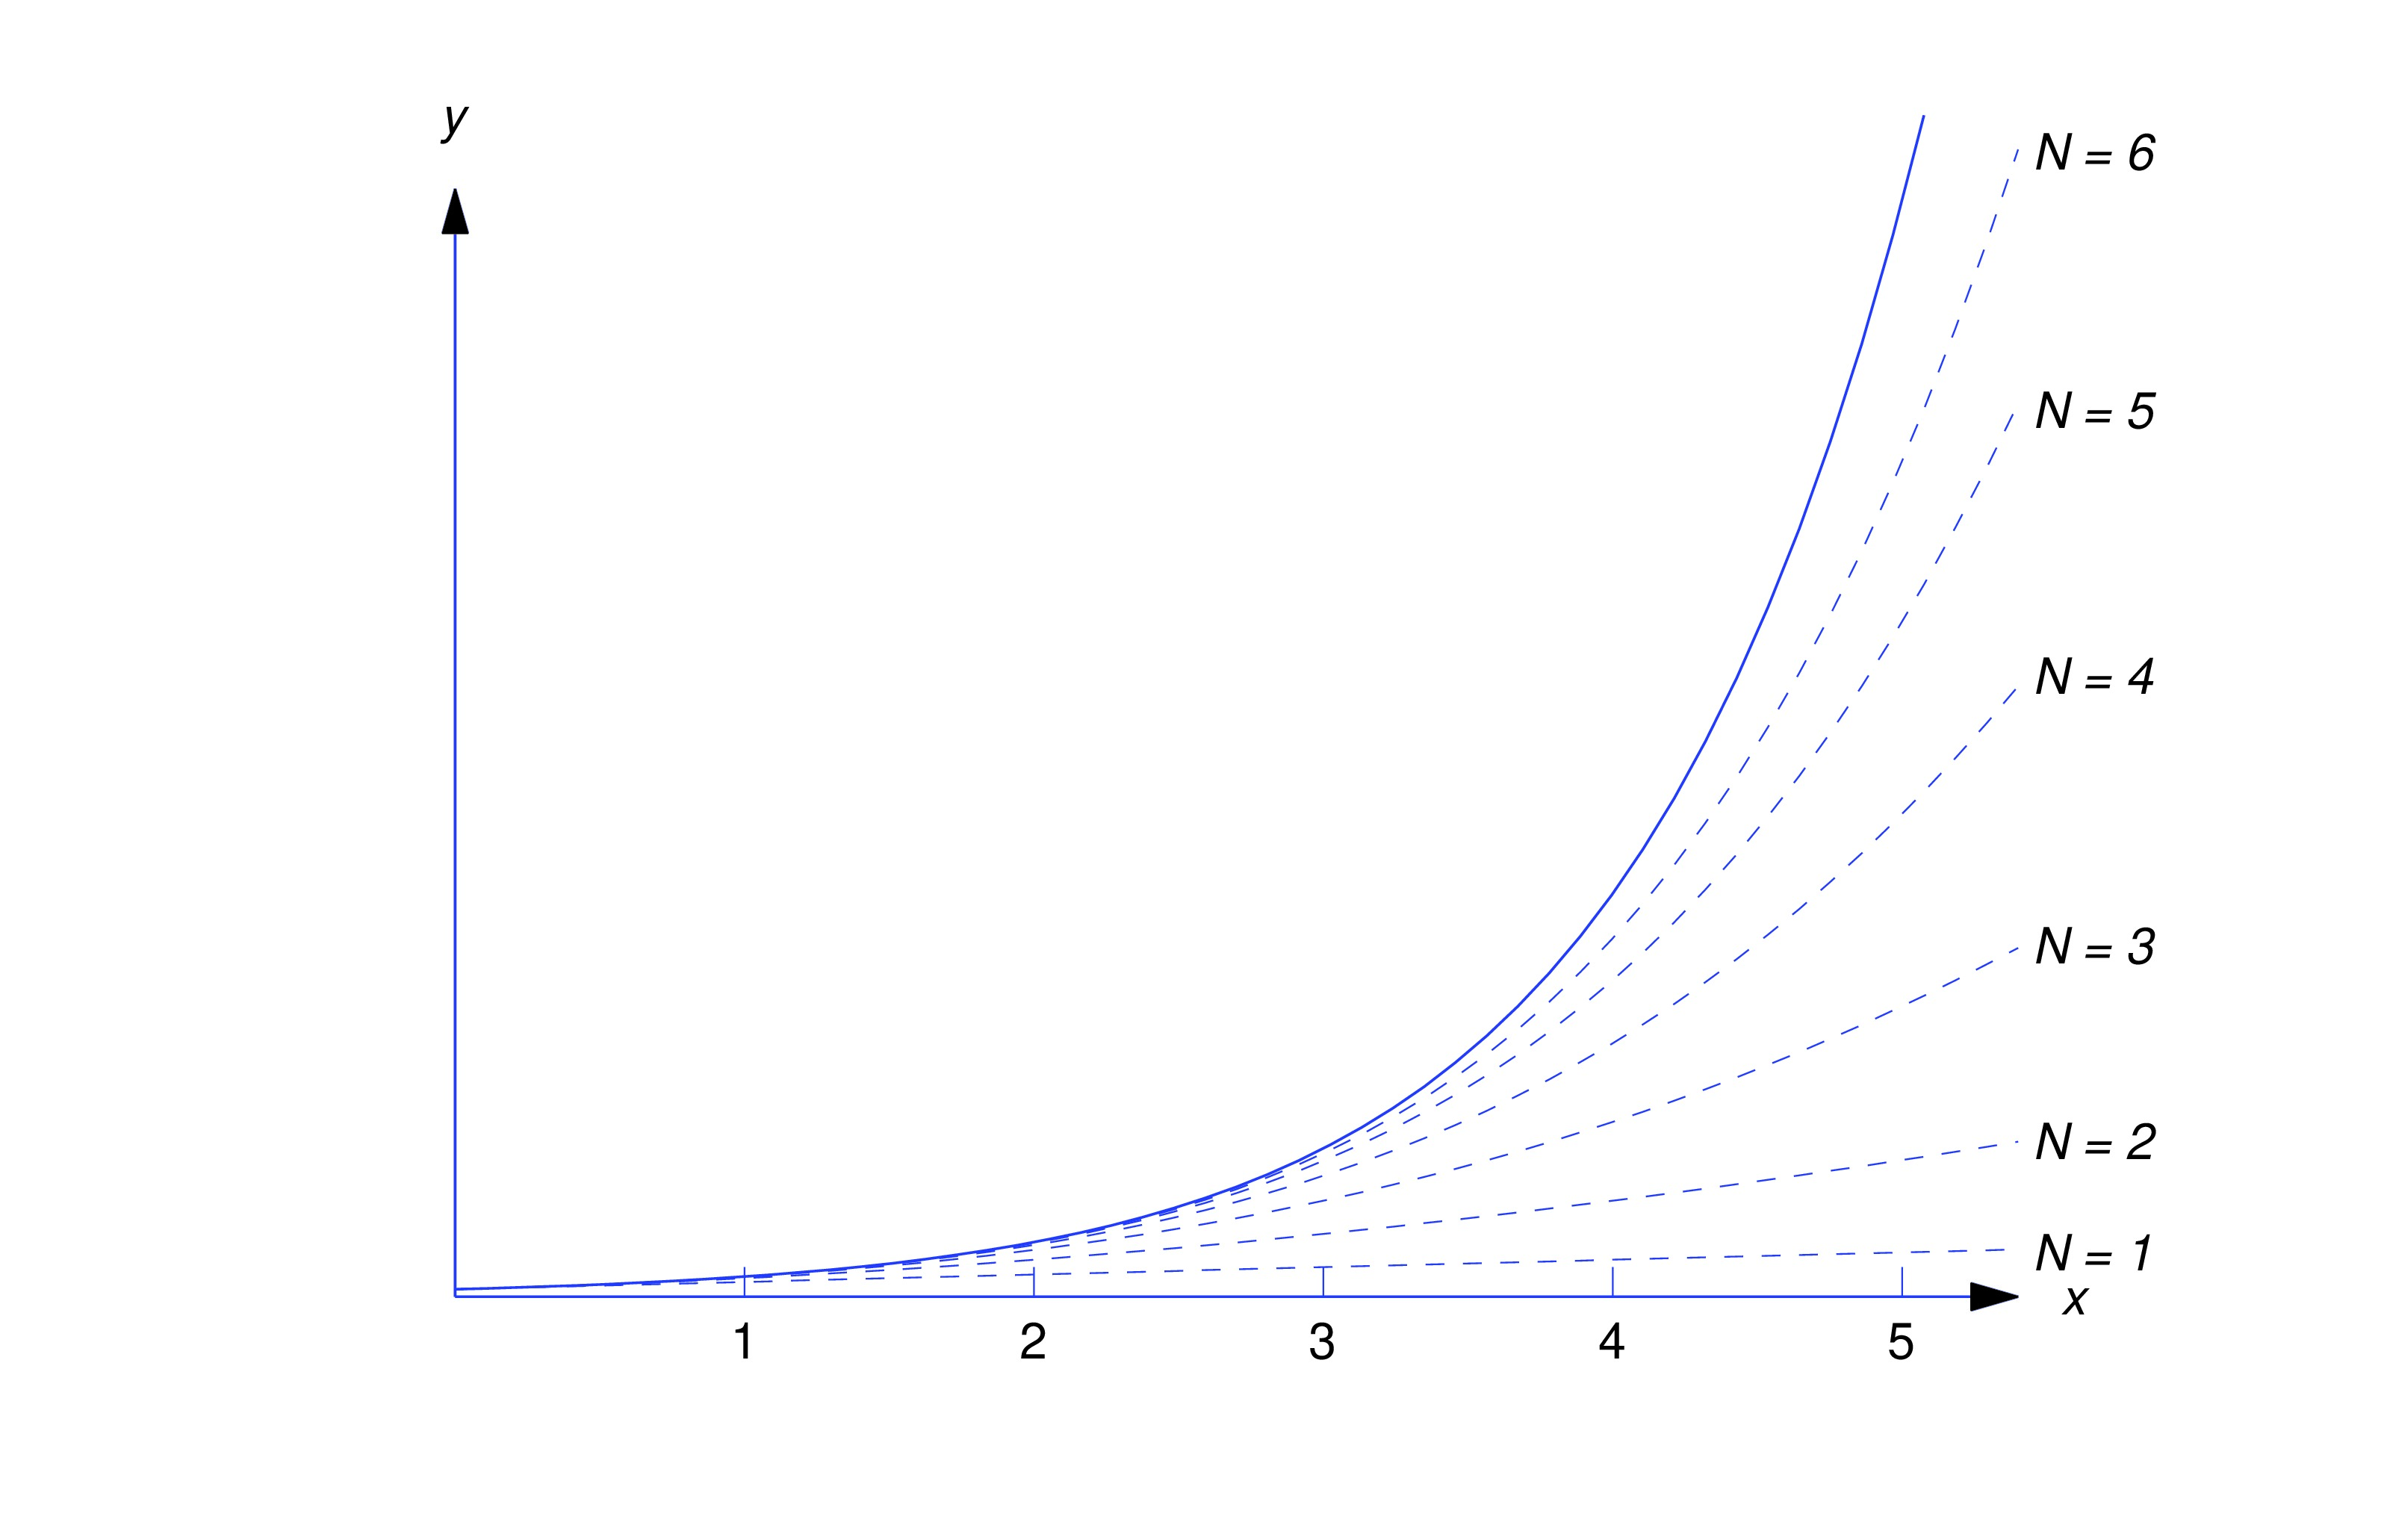
\includegraphics[height=1.5in]{fig070101.jpg} 
\end{image}

From this figure, we conclude
that the accuracy of the
approximation of $y=e^x$ by its Taylor polynomial $T_N$ improves as
$N$ increases.

\subsection*{Shifting the Summation Index}

In Definition~\ref{thmtype:7.1.1} of a power series in $x-x_0$, the $n$-th
term is a constant multiple of $(x-x_0)^n$. This isn't  true in
\eqref{eq:7.1.6}, \eqref{eq:7.1.7}, and \eqref{eq:7.1.8}, where the general
terms are constant multiples of $(x-x_0)^{n-1}$, $(x-x_0)^{n-2}$, and
$(x-x_0)^{n-k}$, respectively. However, these series can all be
rewritten so that their $n$-th terms are constant multiples of
$(x-x_0)^n$. For example, letting $n=k+1$ in the series in
\eqref{eq:7.1.6} yields
\begin{equation} \label{eq:7.1.10}
f'(x)=\sum_{k=0}^\infty (k+1)a_{k+1}(x-x_0)^k,
\end{equation}
where we start the new summation index $k$ from zero so that the first
term in \eqref{eq:7.1.10} (obtained by setting $k=0$) is the same as the
first term in \eqref{eq:7.1.6} (obtained by setting $n=1$). However, the
sum of a series is independent of the symbol used to denote the
summation index, just as the value of a definite integral is
independent of the symbol used to denote the variable of integration.
Therefore we can replace $k$ by $n$ in \eqref{eq:7.1.10} to obtain
\begin{equation} \label{eq:7.1.11}
f'(x)=\sum_{n=0}^\infty (n+1)a_{n+1}(x-x_0)^n,
\end{equation}
where the general term is a  constant multiple of  $(x-x_0)^n$.

It isn't  really necessary to introduce the intermediate summation
index $k$. We can obtain \eqref{eq:7.1.11} directly from \eqref{eq:7.1.6}
by replacing $n$ by $n+1$ in the general term of \eqref{eq:7.1.6} and
subtracting $1$ from the lower limit of \eqref{eq:7.1.6}. More generally,
we use the following procedure for shifting indices.

\begin{procedure}
{\bf Shifting the Summation Index in a Power
Series}

For any integer $k$,  the power series
$$
\sum_{n=n_0}^\infty b_n(x-x_0)^{n-k}
$$
can be rewritten  as
$$
\sum_{n=n_0-k}^\infty b_{n+k}(x-x_0)^n;
$$
that is, replacing $n$ by $n+k$ in the general term and subtracting
$k$ from the lower limit of summation leaves the series unchanged.
\end{procedure}

\begin{example}\label{example:7.1.3}
Rewrite the following power series from \eqref{eq:7.1.7}  and \eqref{eq:7.1.8}
so that the general term in each  is a  constant multiple of
$(x-x_0)^n$:
\begin{enumerate}
    \item \label{item:7.1.3a}
$\sum_{n=2}^\infty
n(n-1)a_n(x-x_0)^{n-2}$
\item \label{item:7.1.3b}
$\sum_{n=k}^\infty
n(n-1)\cdots(n-k+1)a_n(x-x_0)^{n-k}.
$
\end{enumerate}

\begin{explanation}
\ref{item:7.1.3a} Replacing $n$ by $n+2$ in the general term
and subtracting $2$ from the lower limit of summation yields
$$
\sum_{n=2}^\infty n(n-1)a_n(x-x_0)^{n-2}=
\sum_{n=0}^\infty (n+2)(n+1)a_{n+2}(x-x_0)^n.
$$

\ref{item:7.1.3b}  Replacing $n$ by $n+k$ in the general term
and subtracting $k$ from the lower limit of summation yields
$$
\sum_{n=k}^\infty
n(n-1)\cdots(n-k+1)a_n(x-x_0)^{n-k}=
\sum_{n=0}^\infty (n+k)(n+k-1)\cdots(n+1)a_{n+k}(x-x_0)^n.
$$
\end{explanation}
\end{example}

\begin{example}\label{example:7.1.4}
Given that
$$
f(x)=\sum_{n=0}^\infty a_nx^n,
$$
write the function $xf''$  as a power series in which the general term
is a  constant multiple of $x^n$.

\begin{explanation}
From Theorem~\ref{thmtype:7.1.4} with $x_0=0$,
$$
f''(x)=\sum_{n=2}^\infty n(n-1)a_nx^{n-2}.
$$
Therefore
$$
xf''(x)=\sum_{n=2}^\infty n(n-1)a_nx^{n-1}.
$$
Replacing $n$ by $n+1$ in the general term and  subtracting $1$
from the lower limit of summation yields
$$
xf''(x)=\sum_{n=1}^\infty (n+1)na_{n+1}x^n.
$$
We can also write this as
$$
xf''(x)=\sum_{n=0}^\infty (n+1)na_{n+1}x^n,
$$
since the first term in this last series is zero.  (We'll see
later that  sometimes it's useful to include zero terms at the
beginning of a series.)

\end{explanation}
\end{example}

\subsection*{Linear Combinations of Power Series}

If a power series is multiplied by a constant, then the constant can be
placed inside the summation; that is,
$$
c\sum_{n=0}^\infty a_n(x-x_0)^n=\sum_{n=0}^\infty ca_n(x-x_0)^n.
$$
Two power series
$$
f(x)=\sum_{n=0}^\infty a_n(x-x_0)^n\quad\mbox{and}\quad
g(x)=\sum_{n=0}^\infty b_n(x-x_0)^n
$$
with positive radii of convergence can be added term by term at points
common to their open intervals of convergence;   thus, if the first
series converges for $|x-x_0|<R_1$ and the second converges for
$|x-x_0|<R_2$, then
$$
f(x)+g(x)=\sum_{n=0}^\infty(a_n+b_n)(x-x_0)^n
$$
for $|x-x_0|<R$, where $R$ is the smaller of $R_1$ and $R_2$.
More generally, linear combinations of power series can be formed term
by term;   for example,
$$
c_1f(x)+c_2f(x)=\sum_{n=0}^\infty(c_1a_n+c_2b_n)(x-x_0)^n.
$$

\begin{example}\label{example:7.1.5}
Find the Maclaurin series for $\cosh x$  as a linear
combination of the Maclaurin series for $e^x$ and $e^{-x}$.

\begin{explanation}
By definition,
$$
\cosh x=\frac{1}{2}e^x+\frac{1}{2}e^{-x}.
$$
Since
$$ e^x=\sum_{n=0}^\infty  \frac{x^n}{n!}\quad\mbox{and}\quad
 e^{-x}=\sum_{n=0}^\infty (-1)^n \frac{x^n}{n!},
$$
it follows that
\begin{equation} \label{eq:7.1.12}
\cosh x=\sum_{n=0}^\infty \frac{1}{2}[1+(-1)^n]\frac{x^n}{n!}.
\end{equation}
Since
$$
\frac{1}{2}[1+(-1)^n]=\left\{\begin{array}{cl}1&\mbox{ if } n=2m,\mbox{
an even integer},\\ 0&\mbox{ if }n=2m+1,\mbox{ an odd integer},
\end{array}\right.
$$
we can rewrite \eqref{eq:7.1.12} more simply as
$$
\cosh x=\sum_{m=0}^\infty\frac{x^{2m}}{(2m)!}
$$
This result is valid on $(-\infty,\infty)$, since this is the open
interval of convergence of the Maclaurin series for $e^x$ and
$e^{-x}$.
\end{explanation}
\end{example}

\begin{example}\label{example:7.1.6}
Suppose
$$
y=\sum_{n=0}^\infty a_n x^n
$$
 on an open interval $I$ that contains the origin.
\begin{enumerate}
\item\label{item:ex7.1.6a} % (a)
Express
$$
(2-x)y''+2y
$$
as a power series in $x$ on $I$.
\item\label{item:ex7.1.6b} % (b)
Use the result of \ref{item:ex7.1.6a} to find necessary and sufficient conditions
on the coefficients $\{a_n\}$ for
 $y$ to be  a solution of the homogeneous equation
\begin{equation} \label{eq:7.1.13}
(2-x)y''+2y=0
\end{equation}
on $I$.
\end{enumerate}

\begin{explanation}
\ref{item:ex7.1.6a}
From \eqref{eq:7.1.7} with $x_0=0$,
$$
y''=\sum_{n=2}^\infty n(n-1)a_nx^{n-2}.
$$
Therefore
\begin{equation} \label{eq:7.1.14}
\begin{array}{rcl}
(2-x)y''+2y&=&2y''-xy'+2y\\
&=&\sum_{n=2}^\infty 2n(n-1)a_nx^{n-2}
-\sum_{n=2}^\infty n(n-1)a_nx^{n-1}
+\sum_{n=0}^\infty 2a_n x^n.
\end{array}
\end{equation}
To combine the three series we  shift indices in the first two to
make their general terms  constant multiples of $x^n$;   thus,
\begin{equation} \label{eq:7.1.15}
\sum_{n=2}^\infty
2n(n-1)a_nx^{n-2}=\sum_{n=0}^\infty2(n+2)(n+1)a_{n+2}x^n
\end{equation}
and
\begin{equation} \label{eq:7.1.16}
\sum_{n=2}^\infty n(n-1)a_nx^{n-1}=\sum_{n=1}^\infty(n+1)na_{n+1}x^n
=\sum_{n=0}^\infty(n+1)na_{n+1}x^n,
\end{equation}
where we added a zero term in the last series so that when we
substitute from \eqref{eq:7.1.15} and \eqref{eq:7.1.16} into \eqref{eq:7.1.14}
all three series will start with $n=0$;   thus,
\begin{equation} \label{eq:7.1.17}
(2-x)y''+2y=\sum_{n=0}^\infty
[2(n+2)(n+1)a_{n+2}-(n+1)na_{n+1}+2a_n]x^n.
\end{equation}

\ref{item:ex7.1.6b} From   \eqref{eq:7.1.17}
we see that $y$ satisfies \eqref{eq:7.1.13} on $I$ if
\begin{equation} \label{eq:7.1.18}
2(n+2)(n+1)a_{n+2}-(n+1)na_{n+1}+2a_n=0,\quad n=0,1,2, \dots.
\end{equation}
Conversely, Theorem~\ref{thmtype:7.1.6}~\ref{item:7.1.6b} implies that if
$y=\sum_{n=0}^\infty a_nx^n$
satisfies \eqref{eq:7.1.13} on $I$,  then \eqref{eq:7.1.18} holds.
\end{explanation}
\end{example}

\begin{example}\label{example:7.1.7}
Suppose
$$
y=\sum_{n=0}^\infty a_n (x-1)^n
$$
 on an open interval $I$ that contains $x_0=1$.
Express the function
\begin{equation} \label{eq:7.1.19}
(1+x)y''+2(x-1)^2y'+3y
\end{equation}
as a power series in $x-1$ on $I$.

\begin{explanation}  Since we want a  power series in $x-1$,
we rewrite the coefficient of $y''$ in \eqref{eq:7.1.19} as
$1+x=2+(x-1)$, so   \eqref{eq:7.1.19} becomes
$$
2y''+(x-1)y''+2(x-1)^2y'+3y.
$$
From \eqref{eq:7.1.6}  and \eqref{eq:7.1.7} with $x_0=1$,
$$
y'=\sum_{n=1}^\infty na_n(x-1)^{n-1}\quad\mbox{and}\quad
y ''=\sum_{n=2}^\infty n(n-1)a_n(x-1)^{n-2}.
$$
Therefore
\begin{eqnarray*}
2y ''&=&\sum_{n=2}^\infty 2n(n-1)a_n(x-1)^{n-2},\\
(x-1)y ''&=&\sum_{n=2}^\infty n(n-1)a_n(x-1)^{n-1},\\
2(x-1)^2y'&=&\sum_{n=1}^\infty2na_n(x-1)^{n+1},\\
3y&=&\sum_{n=0}^\infty 3a_n (x-1)^n.
\end{eqnarray*}
Before adding these four series we shift indices in the first three so
that their general terms become constant multiples of $(x-1)^n$. This
yields
\begin{eqnarray}
2y ''&=&\sum_{n=0}^\infty 2(n+2)(n+1)a_{n+2}(x-1)^n,\label{eq:7.1.20}\\
(x-1)y''&=&\sum_{n=0}^\infty (n+1)na_{n+1}(x-1)^n,
\label{eq:7.1.21}\\
2(x-1)^2y'&=&\sum_{n=1}^\infty 2(n-1)a_{n-1}(x-1)^n,\label{eq:7.1.22}\\
%dummy \eqref{eq:7.1.22}
3y&=&\sum_{n=0}^\infty 3a_n (x-1)^n, \label{eq:7.1.23}
\end{eqnarray}
where we added initial zero terms to the series in \eqref{eq:7.1.21}
and \eqref{eq:7.1.22}.  Adding \eqref{eq:7.1.20}--\eqref{eq:7.1.23} yields
\begin{eqnarray*}
(1+x)y''+2(x-1)^2y'+3y&=&2y''+(x-1)y''+2(x-1)^2y'+3y\\[5pt]
&=&\sum_{n=0}^\infty  b_n (x-1)^n,
\end{eqnarray*}
where
\begin{eqnarray}
b_0&=&4a_2+3a_0, \label{eq:7.1.24}\\
b_n&=&2(n+2)(n+1)a_{n+2}+(n+1)na_{n+1}+2(n-1)a_{n-1}+3a_n\nonumber
\\
&&n\geq 1\label{eq:7.1.25}.
\end{eqnarray}
The formula \eqref{eq:7.1.24} for $b_0$  can't be obtained by
setting $n=0$ in \eqref{eq:7.1.25}, since the summation in \eqref{eq:7.1.22}
begins with $n=1$,  while those in \eqref{eq:7.1.20}, \eqref{eq:7.1.21},
and \eqref{eq:7.1.23} begin with $n=0$.
\end{explanation}
\end{example}



\section*{Text Source}
Trench, William F., "Elementary Differential Equations" (2013). Faculty Authored and Edited Books \& CDs. 8. (CC-BY-NC-SA)

\href{https://digitalcommons.trinity.edu/mono/8/}{https://digitalcommons.trinity.edu/mono/8/}


\end{document}